\section{Toric Degenerations}
This section compares the toric degeneration from the usual toric boundary with the degeneration selected by the type \(C_n\) flag valuation. In both cases, the degree-one value polytope is the polar dual of the Newton polytope of the corresponding Laurent superpotential.

We use the following convention, compatible with the usual polar-dual convention in toric mirror symmetry \cite{Bat94}. If \(P=\operatorname{Newt}(W)\) is the Newton polytope of a Laurent polynomial and the origin is in its interior, then
\[
P^\vee=\{u:\langle u,v\rangle\ge -1\ \text{for all }v\in P\}.
\]
With this convention, in the examples below the degree-one value set of the valuation is \(P^\vee\).

\subsection{Toric degenerations from valuations}
We recall the valuation mechanism behind the toric degenerations used below. Let \(X\) be a projective variety with an ample line bundle \(L\), and let
\[
R=\bigoplus_{k\ge0}H^0(X,L^k)
\]
be its section ring. A valuation on \(R\), ordered lexicographically on each graded piece, must be combined with the grading to produce the value semigroup. Thus, for \(0\ne s\in H^0(X,L^k)\), we use the degree-augmented value
\[
\widetilde\nu(s)=(k,\nu(s)).
\]
The corresponding value semigroup is
\[
S(R,\nu)=\{(k,\nu(s)):0\ne s\in H^0(X,L^k)\}
\]
in \(\ZZ_{\ge0}\times\ZZ^d\). If the valuation has one-dimensional leaves and this semigroup is finitely generated, then the associated graded algebra is
\[
\operatorname{gr}_\nu R\simeq \CC[S(R,\nu)].
\]
The Rees algebra of the valuation filtration then gives a flat degeneration
\[
X=\operatorname{Proj}R\rightsquigarrow \operatorname{Proj}\operatorname{gr}_\nu R.
\]
The special fibre is therefore the projective toric variety determined by the cone over the Newton--Okounkov body. This is the form of Anderson's Newton--Okounkov toric degeneration theorem used below \cite{Anderson}; see also the foundational constructions of Newton--Okounkov bodies in \cite{KK,LM} and the integrable-systems perspective in \cite{HK}.

A standard way to obtain such a valuation is to choose an admissible flag
\[
X=Y_0\supset Y_1\supset\cdots\supset Y_d=\{p\},
\]
with each \(Y_i\) irreducible and smooth at \(p\). The flag valuation records successive orders of vanishing along \(Y_1,Y_2,\ldots,Y_d\). We first illustrate this in the explicit \(\PP^3\) calculation, then record the standard toric valuation for \(\PP^N\), and finally use the type \(C_n\) flag whose value polytope is the polar dual of the Newton polytope of the Lie-theoretical Laurent polynomial.

\subsection{Toy example: \(\PP^3\)}
Let \(X=\PP^3\) with homogeneous coordinates \([p_0:p_1:p_2:p_3]\). The Lie-theoretical calculation in this example is based on Tillmann-Morris's unpublished mini-project report \cite{TillmannMorris}; Section~6 of the same manuscript also records the odd-dimensional formula used in Theorem~\ref{thm:lusztig-potential}. For the standard toric boundary \(p_0p_1p_2p_3=0\), work on the affine chart \(p_0\ne0\) and write
\[
x=\frac{p_1}{p_0},
\qquad
y=\frac{p_2}{p_0},
\qquad
z=\frac{p_3}{p_0}.
\]
The toric mirror potential (see Example~\ref{ex:tor-PN}) is
\[
W_{xyz}=x+y+z+\frac{1}{xyz}.
\]
Its Newton polytope is
\[
P_{xyz}
=
\operatorname{Conv}\{(1,0,0),(0,1,0),(0,0,1),(-1,-1,-1)\}.
\]
Its polar dual is
\[
P_{xyz}^\vee
=
\{(X,Y,Z)\in\RR^3:
X,Y,Z\ge -1,\ X+Y+Z\le1\}.
\]
This is the usual valuation polytope for the toric degeneration of \(\PP^3\).

On the other hand, the type \(C_2\) Lie-theoretical calculation of Theorem~\ref{thm:lusztig-potential} gives, after setting the quantum parameter \(q=1\) for the purpose of taking the Newton polytope, the Laurent polynomial
\[
W_{abc}
=
a+b+c+\frac{1}{ab^2}+\frac{1}{b^2c}.
\]
The support exponents are
\[
(1,0,0),\quad (0,1,0),\quad (0,0,1),
\quad (-1,-2,0),\quad (0,-2,-1).
\]
Hence, if \(P_{abc}=\operatorname{Newt}(W_{abc})\), then
\[
P_{abc}^\vee
=
\{(A,B,C)\in\RR^3:
A,B,C\ge -1,\ A+2B\le1,\ 2B+C\le1\}.
\]

\begin{rmk}
When \(n=2\), the Laurent polynomial obtained from the type \(C_2\) Lusztig torus is mutation-equivalent to the standard toric Hori--Vafa potential. In the sense of Akhtar--Coates--Galkin--Kasprzyk~\cite{ACGK}, the following birational map is the composition of three Laurent mutations:
\[
a=\frac{xy}{x+z},\qquad
b=x+z,\qquad
c=\frac{yz}{x+z}.
\]
It sends \(W_{xyz}=x+y+z+1/(xyz)\) to \(W_{abc}=a+b+c+1/(ab^2)+1/(b^2c)\). This comparison is included only as motivation and as a link with the MMLP picture for Fano threefolds \cite{CKPT}.
\end{rmk}

The two polytopes in this toy example are shown in Figure~\ref{fig:p3-polytopes}.

\begin{figure}[ht]
\centering
\begin{minipage}{0.47\textwidth}
\centering
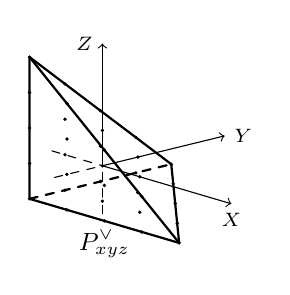
\begin{tikzpicture}[scale=.5,x={(0.95cm,-0.28cm)},y={(0.9cm,0.22cm)},z={(0cm,0.9cm)},line join=round,line cap=round]
\coordinate (O) at (-1,-1,-1);
\coordinate (X) at (3,-1,-1);
\coordinate (Y) at (-1,3,-1);
\coordinate (Z) at (-1,-1,3);
\draw[dashed] (-1.35,0,0)--(0,0,0);
\draw[dashed] (0,-1.35,0)--(0,0,0);
\draw[dashed] (0,0,-1.35)--(0,0,0);
\draw[->] (0,0,0)--(3.45,0,0) node[below] {\scriptsize \(X\)};
\draw[->] (0,0,0)--(0,3.45,0) node[right] {\scriptsize \(Y\)};
\draw[->] (0,0,0)--(0,0,3.45) node[left] {\scriptsize \(Z\)};
\foreach \Xcoord in {-1,0,1,2,3}{
  \foreach \Ycoord in {-1,0,1,2,3}{
    \foreach \Zcoord in {-1,0,1,2,3}{
      \pgfmathtruncatemacro{\scoord}{\Xcoord+\Ycoord+\Zcoord}
      \ifnum\scoord<2
        \fill (\Xcoord,\Ycoord,\Zcoord) circle (1.35pt);
      \fi
    }
  }
}
\draw[thick,dashed] (O)--(Y);
\draw[thick] (O)--(X)--(Y)--(Z)--(O);
\draw[thick] (X)--(Z);
\node[below] at (1,-1,-1) {\small \(P_{xyz}^\vee\)};
\end{tikzpicture}
\end{minipage}
\hfill
\begin{minipage}{0.47\textwidth}
\centering
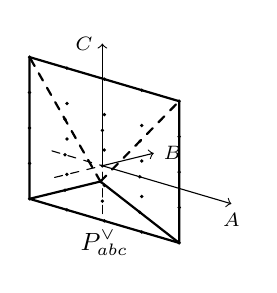
\begin{tikzpicture}[scale=.5,x={(0.95cm,-0.28cm)},y={(0.9cm,0.22cm)},z={(0cm,0.9cm)},line join=round,line cap=round]
\coordinate (O) at (-1,-1,-1);
\coordinate (X) at (3,-1,-1);
\coordinate (Z) at (-1,-1,3);
\coordinate (T) at (-1,1,-1);
\coordinate (U) at (3,-1,3);
\draw[dashed] (-1.35,0,0)--(0,0,0);
\draw[dashed] (0,-1.35,0)--(0,0,0);
\draw[dashed] (0,0,-1.35)--(0,0,0);
\draw[->] (0,0,0)--(3.45,0,0) node[below] {\scriptsize \(A\)};
\draw[->] (0,0,0)--(0,1.45,0) node[right] {\scriptsize \(B\)};
\draw[->] (0,0,0)--(0,0,3.45) node[left] {\scriptsize \(C\)};
\foreach \Acoord in {-1,0,1,2,3}{
  \foreach \Bcoord in {-1,0,1}{
    \foreach \Ccoord in {-1,0,1,2,3}{
      \pgfmathtruncatemacro{\sAcoord}{\Acoord+2*\Bcoord}
      \pgfmathtruncatemacro{\sCcoord}{\Ccoord+2*\Bcoord}
      \ifnum\sAcoord<2
        \ifnum\sCcoord<2
          \fill (\Acoord,\Bcoord,\Ccoord) circle (1.35pt);
        \fi
      \fi
    }
  }
}
\draw[thick,dashed] (T)--(Z);
\draw[thick,dashed] (T)--(U);
\draw[thick] (O)--(X)--(U)--(Z)--(O);
\draw[thick] (O)--(T)--(X);
\node[below] at (1,-1,-1) {\small \(P_{abc}^\vee\)};
\end{tikzpicture}
\end{minipage}
\caption{The polar duals of the Newton polytopes of \(W_{xyz}\) and \(W_{abc}\). The black dots are the lattice points in the degree-one normalized value sets after the indicated lattice coordinate identifications.}
\label{fig:p3-polytopes}
\end{figure}

Let
\[
\phi=p_0p_3-p_1p_2,
\qquad
Q=\{\phi=0\}\subset\PP^3.
\]
Then \(Q\simeq\PP^1\times\PP^1\). Use the Segre parametrization
\[
[p_0:p_1:p_2:p_3]
=
[s_0t_0:s_0t_1:s_1t_0:s_1t_1],
\]
and choose the flag
\[
\PP^3\supset Q\supset \mathcal C\supset p_\infty,
\]
where
\[
\mathcal C=\{s_0=0\}=\{p_0=p_1=0\}\subset Q,
\qquad
p_\infty=[0:0:0:1].
\]
Put
\[
s_\star=p_0p_3\phi=p_0p_3(p_0p_3-p_1p_2).
\]
For \(s\in H^0(\PP^3,\mathcal O(4k))\), write \(r=\operatorname{ord}_Q(s)\), remove the factor \(\phi^r\), and restrict the residual section to \(Q\). If \((i,j)\) is the standard toric flag value on \(Q\simeq\PP^1\times\PP^1\), the original flag valuation is
\[
\nu(s)=(r,i,j).
\]
Let
\[
\sigma:\ZZ^3\longrightarrow\ZZ^3,
\qquad
\sigma(r,i,j)=(i,r,j).
\]
For \(0\ne s\in H^0(\PP^3,\mathcal O(4k))\), define the normalized lattice-labelled value
\[
\lambda_{abc,k}(s)
:=
\sigma\bigl(\nu(s)-k\mathbf 1\bigr),
\qquad
\mathbf 1=(1,1,1).
\]
Thus
\[
\lambda_{abc,k}(s)
=
(i-k,\ r-k,\ j-k).
\]
The map \(\sigma\) is used only to identify the flag-value lattice with the exponent lattice of \(W_{abc}\). We do not equip the reordered coordinates with the standard lexicographic order and regard the resulting map as a new valuation.
The degree \(k\) normalized value set is
\[
\left\{
\lambda_{abc,k}(s):
0\ne s\in H^0(\PP^3,\mathcal O(4k))
\right\}
=
kP_{abc}^{\vee}\cap\ZZ^3.
\]
To see this directly, use a basis adapted to the filtration by powers of \(\phi\). For \(0\le r\le 2k\), put \(d=4k-2r\). Restriction identifies the \(r\)-th associated graded quotient with \(H^0(Q,\mathcal O_Q(d,d))\). On \(Q\simeq\PP^1\times\PP^1\), the monomials \(s_0^is_1^{d-i}t_0^jt_1^{d-j}\), \(0\le i,j\le d\), have toric flag values \((i,j)\). After choosing homogeneous lifts, the adapted basis elements have normalized values \((i-k,r-k,j-k)\), where \(0\le r\le2k\) and \(0\le i,j\le4k-2r\). Thus the degree \(k\) value set is cut out by \(A,B,C\ge-k\), \(A+2B\le k\), and \(2B+C\le k\). Therefore
\[
\left\{
\lambda_{abc,k}(s):
0\ne s\in H^0(\PP^3,\mathcal O(4k))
\right\}
=
kP_{abc}^\vee\cap\ZZ^3.
\]

\begin{exam}
Take \(s=\phi\,p_0^2\). Then \(k=1\), \(r=1\), and \(p_0^2|_Q=(s_0t_0)^2\), so the toric flag value on \(Q\simeq\PP^1\times\PP^1\) is \((i,j)=(2,2)\). Hence \(\lambda_{abc,1}(s)=(1,0,1)\), which lies on the two facets \(A+2B=1\) and \(2B+C=1\) of \(P_{abc}^\vee\). This agrees with the case \(n=2\) of the general construction below, since \(\phi=-F_1\).
\end{exam}

\subsection{The standard toric valuation}
We now record the analogous valuation for the classical toric mirror of \(\PP^N\). Let \(H_{\mathrm{tor}}=p_0p_1\cdots p_N\) be the toric anticanonical section. The anticanonical section ring is \(R_{\mathrm{tor}}=\bigoplus_{k\ge0}H^0(\PP^N,\mathcal O((N+1)k))\). On the affine chart \(p_0\ne0\), set \(x_i=p_i/p_0\) for \(1\le i\le N\).
After dividing a degree \((N+1)k\) section by \(H_{\mathrm{tor}}^k\), it becomes a Laurent polynomial in the \(x_i\)'s. We use the monomial valuation
\[
\nu_{\mathrm{tor}}\left(\sum_m c_mx^m\right)
=
\min_{\mathrm{lex}}\{m\in\ZZ^N:c_m\ne0\},
\]
so that \(\nu_{\mathrm{tor}}(x^m)=m\). This is the valuation obtained by recording the exponent vector in the standard torus coordinates.

Let
\[
P_{\mathrm{tor}}^{(N)}
=
\operatorname{Newt}\left(x_1+\cdots+x_N+\frac{q}{x_1\cdots x_N}\right)
=
\operatorname{Conv}\{e_1,\ldots,e_N,-\mathbf 1\},
\]
where \(\mathbf 1=(1,\ldots,1)\).

\begin{thm}\label{thm:standard-toric-valuation}
For every \(k\ge0\),
\[
\left\{
\nu_{\mathrm{tor}}\left(\frac{s}{H_{\mathrm{tor}}^k}\right):
0\ne s\in H^0(\PP^N,\mathcal O((N+1)k))
\right\}
=
k\bigl(P_{\mathrm{tor}}^{(N)}\bigr)^\vee\cap\ZZ^N.
\]
If \(\widetilde\nu_{\mathrm{tor}}(s)=(k,\nu_{\mathrm{tor}}(s/H_{\mathrm{tor}}^k))\), then the corresponding Rees algebra gives the standard toric degeneration associated with the polar dual of the Newton polytope of the classical toric mirror.
\end{thm}

\begin{proof}
Use the standard monomial basis of \(H^0(\PP^N,\mathcal O((N+1)k))\):
\[
p^\alpha=p_0^{\alpha_0}p_1^{\alpha_1}\cdots p_N^{\alpha_N},
\qquad
|\alpha|=(N+1)k.
\]
On the chart \(p_0\ne0\), we have
\[
\frac{p^\alpha}{H_{\mathrm{tor}}^k}
=
x_1^{\alpha_1-k}\cdots x_N^{\alpha_N-k}.
\]
Thus its value is
\[
m=(\alpha_1-k,\ldots,\alpha_N-k).
\]
The conditions \(\alpha_i\ge0\) for \(1\le i\le N\) give \(m_i\ge-k\). The remaining condition
\(\alpha_0=(N+1)k-\sum_{i=1}^N\alpha_i\ge0\) gives \(\sum_i m_i\le k\). Conversely, any integral \(m\) satisfying these inequalities is obtained by setting
\[
\alpha_i=m_i+k\quad(1\le i\le N),
\qquad
\alpha_0=k-\sum_{i=1}^Nm_i.
\]
Since the lexicographic monomial valuation of a nonzero linear combination is the value of one of its monomial terms, the degree \(k\) value set is exactly
\[
\left\{
\nu_{\mathrm{tor}}\left(\frac{s}{H_{\mathrm{tor}}^k}\right):
0\ne s\in H^0(\PP^N,\mathcal O((N+1)k))
\right\}
=
\{m\in\ZZ^N:m_i\ge-k,\ \sum_i m_i\le k\}.
\]

On the other hand, \(P_{\mathrm{tor}}^{(N)}=\operatorname{Conv}\{e_1,\ldots,e_N,-\mathbf 1\}\). By the polar convention fixed at the beginning of this section, \(\bigl(P_{\mathrm{tor}}^{(N)}\bigr)^\vee\) is cut out by
\[
u_i\ge -1\qquad(1\le i\le N),
\qquad
\sum_{i=1}^Nu_i\le1.
\]
Thus
\[
k\bigl(P_{\mathrm{tor}}^{(N)}\bigr)^\vee\cap\ZZ^N
=
\{m\in\ZZ^N:m_i\ge-k,\ \sum_i m_i\le k\},
\]
which is exactly the value set computed above.

After adjoining the degree, the value semigroup is
\[
S_{\mathrm{tor}}
=
\{(k,m):k\ge0,\ m\in k(P_{\mathrm{tor}}^{(N)})^\vee\cap\ZZ^N\}.
\]
It is finitely generated by Gordan's lemma, and the monomial valuation has one-dimensional leaves. Anderson's Newton--Okounkov theorem therefore gives a flat Rees degeneration with special fibre \(\operatorname{Proj}\CC[S_{\mathrm{tor}}]\), the projective toric variety associated with \((P_{\mathrm{tor}}^{(N)})^\vee\).
\end{proof}

\subsection{The flag valuation and the Newton--Okounkov body}
Let \(X=\PP^{2n-1}\) with homogeneous coordinates \([p_0:\cdots:p_N]\), where \(N=2n-1\). In the previous section the type \(C_n\) boundary \(D_C\) was defined by \(H_N=p_0p_N\prod_{r=1}^{n-1}F_r\), with \(F_r=\sum_{j=0}^r(-1)^jp_{r-j}p_{N-r+j}\).
The following flag and valuation generalize the type \(C\) calculation. They give the valuation-side construction of the toric degeneration adapted to the type \(C_n\) anticanonical section \(H_N\).
Set \(F_0=p_0p_N\). Then, for \(1\le r\le n-1\), \(F_r=p_rp_{N-r}-F_{r-1}\).
Let \(Q_r=\{F_r=0\}\). The flag used below starts with \(Y_0=\PP^N\) and \(Y_1=Q_{n-1}\). Then, for \(m=n-1,n-2,\ldots,2\), impose successively the two hyperplane conditions \(p_m=0\) and \(p_{N-m}=0\).
After these steps the remaining surface is
\[
Q_1=\{p_1p_{N-1}-p_0p_N=0\}
\subset \PP\langle p_0,p_1,p_{N-1},p_N\rangle\cong \PP^3.
\]
This is a smooth quadric surface. Identify it with \(\PP^1\times\PP^1\) by
\[
p_0=X_0Y_0,
\qquad
p_1=X_1Y_0,
\qquad
p_{N-1}=X_0Y_1,
\qquad
p_N=X_1Y_1.
\]
On \(Q_1\), finish the flag by taking
\[
C=\{Y_0=0\}=\{p_0=p_1=0\}
\]
and
\[
p_\infty=([0:1],[0:1])=[0:\cdots:0:1].
\]
Let \(Y_\bullet\) denote the resulting full flag. Near \(p_\infty\), with local coordinates
\[
x=\frac{X_0}{X_1}=\frac{p_{N-1}}{p_N},
\qquad
 y=\frac{Y_0}{Y_1}=\frac{p_1}{p_N},
\]
the final flag is \(Q_1\supset\{y=0\}\supset\{x=y=0\}\).

\begin{lemma}\label{lem:flag-admissible}
The flag \(Y_\bullet\) is admissible: every member is irreducible and smooth at \(p_\infty\), and \(Y_i\) has codimension \(i\) in \(\PP^N\).
\end{lemma}

\begin{proof}
For \(1\le m\le n-1\), set
\[
P_m:=\PP\langle p_0,\ldots,p_m,p_{N-m},\ldots,p_N\rangle
\]
and
\[
Z_m:=\{F_m=0\}\subset P_m.
\]
The quadratic form \(F_m\) is nondegenerate on the coordinates of \(P_m\), so \(Z_m\) is an irreducible quadric for every \(m\ge1\).
The identity
\[
F_m=p_mp_{N-m}-F_{m-1}
\]
is the key point.  Inside \(Z_m\), the intersection with \(p_m=0\) is cut out in \(P_m\) by
\[
p_m=0,\qquad F_{m-1}=0,
\]
while \(p_{N-m}\) remains a free homogeneous coordinate. Hence \(Z_m\cap\{p_m=0\}\) is the projective cone over \(Z_{m-1}\) with vertex in the \(p_{N-m}\)-direction, and is therefore irreducible. Intersecting further with \(p_{N-m}=0\) gives \(Z_{m-1}\subset P_{m-1}\). Together with the irreducibility of the quadrics \(Z_m\), this proves irreducibility of every stratum in the flag and also gives the expected codimensions.

For smoothness at \(p_\infty=[0:\cdots:0:1]\), work in the affine chart \(p_N=1\), with local coordinates \(p_0,\ldots,p_{N-1}\). With the present indexing,
\[
F_m=(-1)^mp_0+\text{terms of order at least }2
\qquad\text{at }p_\infty.
\]
Thus \(F_m\) may replace \(p_0\) as one element of a regular system of parameters in the local ring at \(p_\infty\). At the stage indexed by \(m\), the local equations are \(F_m\) together with the coordinate functions already imposed, namely \(p_{m+1},p_{N-m-1},\ldots,p_{n-1},p_n\), and then successively \(p_m\) and \(p_{N-m}\). These equations have independent linear parts after replacing \(p_0\) by \(F_m\). At the final surface \(Q_1\), the last two equations are \(p_1=0\) and \(p_{N-1}=0\), equivalently \(y=0\) and \(x=0\) in the coordinates on \(Q_1\simeq\PP^1\times\PP^1\). Hence the equations defining every stratum form part of a regular system of parameters at \(p_\infty\), so every stratum is smooth there.
\end{proof}

Let
\[
R=\bigoplus_{k\ge0}H^0(\PP^N,\mathcal O_{\PP^N}((N+1)k)).
\]
Set \(d=2n-1\), and let \(\mathbf 1=(1,\ldots,1)\in\ZZ^d\).
For \(s\in H^0(\PP^N,\mathcal O((N+1)k))\), let
\[
\nu_{\mathrm{flag}}(s)=(r,u_{n-1},v_{n-1},\ldots,u_2,v_2,u_1,v_1)
\]
be the flag valuation just described. Thus \(r\) is the order along \(Q_{n-1}\); for \(2\le m\le n-1\), the pair \((u_m,v_m)\) records the successive orders along \(p_m=0\) and \(p_{N-m}=0\); and \((u_1,v_1)\) is the toric flag valuation on \(Q_1\simeq\PP^1\times\PP^1\), with \(u_1=\operatorname{ord}_C\) and \(v_1=\operatorname{ord}_{p_\infty}\) after restricting to \(C\).

For
\[
H_N=p_0p_N\prod_{r=1}^{n-1}F_r,
\]
one has
\[
\nu_{\mathrm{flag}}(H_N)=\mathbf 1.
\]
Indeed, \(F_{n-1}\) gives the first order, and the identity \(F_r=p_rp_{N-r}-F_{r-1}\) shows inductively that, after restricting to \(Q_r\), the previous factor \(F_{r-1}\) restricts to \(p_rp_{N-r}\). At the last step, \(p_0p_N\) restricts on \(Q_1\) to the local monomial \(xy\), which has final valuation \((1,1)\).

For \(0\ne s\in H^0(\PP^N,\mathcal O((N+1)k))\), define the raw normalized value vector
\[
\lambda_k(s):=\nu_{\mathrm{flag}}(s)-k\mathbf 1.
\]
Write the shifted coordinates as
\[
B=r-k,
\qquad
A_m=u_m-k,
\qquad
C_m=v_m-k
\quad(1\le m\le n-1).
\]
Thus
\[
\lambda_k(s)
=
(B,A_{n-1},C_{n-1},\ldots,A_1,C_1).
\]

\begin{rmk}\label{rmk:lattice-identification}
The Lusztig monomial coordinates use the opposite order for the \(A_m,C_m\)-pairs. To compare value vectors with those exponent coordinates, let \(\sigma:\ZZ^d\longrightarrow\ZZ^d\) be the lattice permutation \(\sigma(B,A_{n-1},C_{n-1},\ldots,A_1,C_1)=(B,A_1,C_1,\ldots,A_{n-1},C_{n-1})\).
The map \(\sigma\) is only a lattice coordinate identification. We do not regard \(\sigma\circ\lambda_k\), with the standard lexicographic order on the target coordinates after applying \(\sigma\), as a new valuation.

On the degree-augmented lattice define
\[
\Sigma:\ZZ\times\ZZ^d\longrightarrow\ZZ\times\ZZ^d,
\qquad
\Sigma(k,v)=\bigl(k,\sigma(v-k\mathbf 1)\bigr).
\]
For \((k,v),(\ell,w)\in\ZZ\times\ZZ^d\),
\[
\begin{aligned}
\Sigma\bigl((k,v)+(\ell,w)\bigr)
&=
\Sigma(k+\ell,v+w)\\
&=
\bigl(k+\ell,\sigma(v+w-(k+\ell)\mathbf 1)\bigr)\\
&=
\bigl(k+\ell,\sigma(v-k\mathbf 1)+\sigma(w-\ell\mathbf 1)\bigr)\\
&=
\Sigma(k,v)+\Sigma(\ell,w).
\end{aligned}
\]
Thus \(\Sigma\) is a group homomorphism. Its inverse is
\[
\Sigma^{-1}(k,m)=\bigl(k,\sigma^{-1}(m)+k\mathbf 1\bigr),
\]
so \(\Sigma\) is a unimodular lattice automorphism. The toric degeneration below is defined by the original flag valuation; \(\sigma\) and \(\Sigma\) are used only to identify lattice coordinates and value semigroups.
\end{rmk}

With the polar convention fixed above, in the coordinates
\[
(B,A_1,C_1,\ldots,A_{n-1},C_{n-1}),
\]
the polar polytope attached to the type \(C_n\) Lie-theoretical support is
\[
P_n^\vee=\left\{(B,A_1,C_1,\ldots,A_{n-1},C_{n-1})\in\RR^{2n-1}:
\begin{array}{l}
B\ge -1,\ A_m\ge -1,\ C_m\ge -1,\\
A_1+2B+\sum_{m=2}^{n-1}(A_m+C_m)\le1,\\
C_1+2B+\sum_{m=2}^{n-1}(A_m+C_m)\le1
\end{array}
\right\}.
\]
Equivalently, \(P_n^\vee\) is defined by
\[
B\ge -1,
\qquad
A_m\ge -1,
\qquad
C_m\ge -1
\quad(1\le m\le n-1),
\]
and
\[
A_1+2B+\sum_{m=2}^{n-1}(A_m+C_m)\le1,
\]
\[
C_1+2B+\sum_{m=2}^{n-1}(A_m+C_m)\le1.
\]

\begin{prop}\label{prop:no-body-p2n}
For every \(k\ge0\),
\[
\sigma\left(
\left\{
\nu_{\mathrm{flag}}(s)-k\mathbf 1:
0\ne s\in H^0(\PP^N,\mathcal O((N+1)k))
\right\}
\right)
=
kP_n^\vee\cap\ZZ^d.
\]
\end{prop}

\begin{proof}
Let \(s\in H^0(\PP^N,\mathcal O((N+1)k))\), and write
\[
\nu_{\mathrm{flag}}(s)=(r,u_{n-1},v_{n-1},\ldots,u_2,v_2,u_1,v_1).
\]
Write \(B=r-k\), \(A_m=u_m-k\), and \(C_m=v_m-k\).
All entries of \(\nu_{\mathrm{flag}}(s)\) are nonnegative. After removing \(r\) copies of \(F_{n-1}\), the residual degree is \((N+1)k-2r\). After imposing the successive orders \(u_m,v_m\) for \(2\le m\le n-1\), the residual degree on the final quadric \(Q_1\) is
\[
\delta=(N+1)k-2r-
\sum_{m=2}^{n-1}(u_m+v_m).
\]
The restriction of \(\mathcal O_{\PP^N}(\delta)\) to \(Q_1\simeq\PP^1\times\PP^1\) is \(\mathcal O_{Q_1}(\delta,\delta)\). For the standard toric flag on \(\PP^1\times\PP^1\), the value \((u_1,v_1)\) of a section of \(\mathcal O(\delta,\delta)\) satisfies
\[
0\le u_1\le \delta,
\qquad
0\le v_1\le \delta.
\]
Substituting
\[
r=B+k,
\qquad
u_m=A_m+k,
\qquad
v_m=C_m+k
\]
turns these two upper bounds into
\[
A_1+k
\le
(N+1)k-2(B+k)
-
\sum_{m=2}^{n-1}(A_m+C_m+2k).
\]
Since \(N+1=2n\), the constant terms on the right simplify as
\[
(N+1)k-2k-2(n-2)k=2k.
\]
Thus the displayed inequality is equivalent to
\[
A_1+2B+
\sum_{m=2}^{n-1}(A_m+C_m)\le k,
\]
and the same calculation with \(C_1+k\le \delta\) gives
\[
C_1+2B+
\sum_{m=2}^{n-1}(A_m+C_m)\le k.
\]
The nonnegativity of the unshifted valuation entries gives
\[
B\ge -k,
\qquad
A_m\ge -k,
\qquad
C_m\ge -k.
\]
Thus every value vector after applying \(\sigma\) lies in \(kP_n^\vee\cap\ZZ^d\).

Conversely, take any integral point
\[
(B,A_1,C_1,\ldots,A_{n-1},C_{n-1})\in kP_n^\vee\cap\ZZ^d.
\]
Set
\[
r=B+k,
\qquad
u_m=A_m+k,
\qquad
v_m=C_m+k
\quad(1\le m\le n-1).
\]
The lower-bound inequalities imply that all these integers are nonnegative. Define
\[
\delta=(N+1)k-2r-
\sum_{m=2}^{n-1}(u_m+v_m).
\]
The two upper-bound inequalities are precisely
\[
0\le u_1\le \delta,
\qquad
0\le v_1\le \delta.
\]
On \(Q_1\simeq\PP^1\times\PP^1\), choose the section
\[
\sigma_{u_1,v_1}
=
X_0^{v_1}X_1^{\delta-v_1}Y_0^{u_1}Y_1^{\delta-u_1}
\in H^0(Q_1,\mathcal O_{Q_1}(\delta,\delta)).
\]
In the local coordinates \(x=X_0/X_1\), \(y=Y_0/Y_1\) at \(p_\infty\), this section is \(x^{v_1}y^{u_1}\) times a unit, so its toric flag valuation is \((u_1,v_1)\).

Let
\[
L=\PP\langle p_0,p_1,p_{N-1},p_N\rangle\cong\PP^3.
\]
The exact sequence
\[
0\to\mathcal O_L(\delta-2)\to\mathcal O_L(\delta)\to\mathcal O_{Q_1}(\delta,\delta)\to0
\]
and the vanishing \(H^1(L,\mathcal O_L(\delta-2))=0\) for \(\delta\ge0\) show that the restriction map
\[
H^0(L,\mathcal O_L(\delta))\longrightarrow H^0(Q_1,\mathcal O_{Q_1}(\delta,\delta))
\]
is surjective. Choose a homogeneous lift \(\widetilde\sigma\in H^0(L,\mathcal O_L(\delta))\) of \(\sigma_{u_1,v_1}\), and regard it as a homogeneous polynomial in \(p_0,p_1,p_{N-1},p_N\), hence as a section on \(\PP^N\).

Now define
\[
s=
F_{n-1}^r
\left(\prod_{m=2}^{n-1}p_m^{u_m}p_{N-m}^{v_m}\right)
\widetilde\sigma.
\]
Its degree is
\[
2r+
\sum_{m=2}^{n-1}(u_m+v_m)+\delta
=
(N+1)k.
\]
The successive orders are exact. First, \(F_{n-1}\) does not divide the residual factor after removing \(F_{n-1}^r\). Indeed, \(F_{n-1}\) is an irreducible quadratic and is not a coordinate hyperplane factor, so it cannot divide the coordinate monomial part. For \(n>2\), it also cannot divide \(\widetilde\sigma\), since \(\widetilde\sigma\) only uses the final variables \(p_0,p_1,p_{N-1},p_N\), whereas \(F_{n-1}\) contains the term \(p_{n-1}p_n\). For \(n=2\), divisibility by \(F_1\) would force \(\widetilde\sigma|_{Q_1}=0\), contradicting the choice of the nonzero section \(\sigma_{u_1,v_1}\). Hence the order along \(Q_{n-1}\) is \(r\).

For the intermediate orders, argue recursively. Suppose the steps with indices larger than \(m\) have already been passed. The current stratum is \(Z_m=\{F_m=0\}\subset P_m\), and the remaining section has the form
\[
p_m^{u_m}p_{N-m}^{v_m}
\left(\prod_{\ell=2}^{m-1}p_\ell^{u_\ell}p_{N-\ell}^{v_\ell}\right)
\widetilde\sigma
\]
up to a unit along the generic point of the current stratum. On \(Z_m\), the next member of the flag is the divisor \(p_m=0\). Hence \(p_m\) is the local equation whose order is measured at this step. The other displayed factors are not identically zero along the generic point of \(Z_m\cap\{p_m=0\}\): in particular, \(p_{N-m}\) remains free there, and the lower-index coordinates have not yet been imposed. Thus the order along \(p_m=0\) is \(u_m\).

After dividing by \(p_m^{u_m}\) and restricting to \(Z_m\cap\{p_m=0\}\), the identity
\[
F_m=p_mp_{N-m}-F_{m-1}
\]
shows that this intermediate stratum is the projective cone over \(Z_{m-1}\), with \(p_{N-m}\) a Cartier coordinate on the cone direction. The next member of the flag is obtained by imposing \(p_{N-m}=0\). Hence \(p_{N-m}^{v_m}\) contributes order \(v_m\), and after dividing by this power and restricting to \(p_{N-m}=0\), the current stratum becomes \(Z_{m-1}\). Repeating this argument for \(m=n-1,n-2,\ldots,2\) gives all intermediate orders. The lift \(\widetilde\sigma\) uses only the final variables \(p_0,p_1,p_{N-1},p_N\), so it introduces no additional vanishing along these intermediate branches. Finally, \(\sigma_{u_1,v_1}\) was chosen to have toric flag value \((u_1,v_1)\) on \(Q_1\simeq\PP^1\times\PP^1\).

It follows that the successive restrictions along the flag have orders
\[
(r,u_{n-1},v_{n-1},\ldots,u_2,v_2,u_1,v_1).
\]
Thus
\[
\sigma\bigl(\nu_{\mathrm{flag}}(s)-k\mathbf 1\bigr)
=
(B,A_1,C_1,\ldots,A_{n-1},C_{n-1}),
\]
which is the prescribed lattice point after the lattice identification \(\sigma\). Hence every lattice point of \(kP_n^\vee\) occurs.
\end{proof}

\begin{thm}\label{thm:no-toric-degeneration}
Let
\[
S_{\mathrm{flag}}
=
\left\{
\bigl(k,\nu_{\mathrm{flag}}(s)\bigr):
k\ge0,\ 0\ne s\in R_k
\right\},
\qquad
R_k=H^0(\PP^N,\mathcal O((N+1)k)).
\]
Let
\[
S_n=\{(k,m):k\ge0,\ m\in kP_n^\vee\cap\ZZ^d\}.
\]
Then
\[
\Sigma(S_{\mathrm{flag}})=S_n.
\]
Moreover,\footnote{Here and below, \(\operatorname{gr}_{\nu_{\mathrm{flag}}}R\) denotes the associated graded algebra for the filtration on the graded ring \(R\) induced by the degree-augmented value \(0\ne s\in R_k\mapsto(k,\nu_{\mathrm{flag}}(s))\). We retain the shorter notation because the degree is already recorded by the grading of \(R\).}
\[
\operatorname{gr}_{\nu_{\mathrm{flag}}}R
\simeq \CC[S_{\mathrm{flag}}]\simeq \CC[S_n].
\]
The Rees algebra of the filtration defined by the original flag valuation gives a flat degeneration
\[
\PP^N\rightsquigarrow X_{P_n^\vee}:=\operatorname{Proj}\CC[S_n].
\]
The special fibre is the projective toric variety associated with the semigroup cone over \(P_n^\vee\).
\end{thm}

\begin{proof}
The flag is admissible by Lemma~\ref{lem:flag-admissible}, so the associated flag valuation has one-dimensional leaves. The degree-augmented valuation \(s\mapsto(k,\nu_{\mathrm{flag}}(s))\) also has one-dimensional leaves: the degree separates the homogeneous pieces, and within each fixed degree the valuation is the original flag valuation.

For \(0\ne s\in R_k\),
\[
\Sigma\bigl(k,\nu_{\mathrm{flag}}(s)\bigr)
=
\bigl(k,\sigma(\nu_{\mathrm{flag}}(s)-k\mathbf 1)\bigr).
\]
Proposition~\ref{prop:no-body-p2n} identifies the second component, for fixed \(k\), with \(kP_n^\vee\cap\ZZ^d\). Hence \(\Sigma(S_{\mathrm{flag}})=S_n\).

Since \(\Sigma\) is a semigroup isomorphism, it induces an isomorphism of semigroup algebras
\[
\CC[S_{\mathrm{flag}}]\longrightarrow \CC[S_n],
\qquad
\chi^{(k,v)}\longmapsto \chi^{\Sigma(k,v)}.
\]
The semigroup \(S_n\) is the semigroup of lattice points in the rational polyhedral cone over \(P_n^\vee\), so it is finitely generated by Gordan's lemma. Therefore \(S_{\mathrm{flag}}\) is finitely generated as well. Anderson's Newton--Okounkov degeneration theorem applied to the original flag-valuation filtration gives a flat Rees degeneration with general fibre \(R\) and special fibre
\[
\operatorname{gr}_{\nu_{\mathrm{flag}}}R\simeq\CC[S_{\mathrm{flag}}]\simeq\CC[S_n].
\]
Taking \(\operatorname{Proj}\) gives the stated toric degeneration.
\end{proof}

\begin{cor}
Let
\[
W_n:=\left.W_{\mathrm{Lus}}^{(2n-1)}\right|_{q=1}
=
b+
\sum_{m=1}^{n-1}(a_m+c_m)
+
\frac{1}{a_2\cdots a_{n-1}b^2c_{n-1}\cdots c_1}
+
\frac{1}{a_1\cdots a_{n-1}b^2c_{n-1}\cdots c_2},
\]
where an empty product is understood to be \(1\). Then
\[
\operatorname{Newt}(W_n)^\vee=P_n^\vee.
\]
The toric special fibre in Theorem~\ref{thm:no-toric-degeneration} is the projective toric variety whose normal fan is the face fan of \(\operatorname{Newt}(W_n)\).
\end{cor}

\begin{proof}
Expanding the final term of \(W_{\mathrm{Lus}}^{(2n-1)}\) at \(q=1\) gives
\[
\frac{a_1+c_1}
{a_1\cdots a_{n-1}b^2c_{n-1}\cdots c_1}
=
\frac{1}
{a_2\cdots a_{n-1}b^2c_{n-1}\cdots c_1}
+
\frac{1}
{a_1\cdots a_{n-1}b^2c_{n-1}\cdots c_2}.
\]
The exponent vectors of these two monomials, together with those of \(b\), \(a_m\), and \(c_m\), give precisely the inequalities defining \(P_n^\vee\). Hence \(\operatorname{Newt}(W_n)^\vee=P_n^\vee\). The final assertion follows from Theorem~\ref{thm:no-toric-degeneration}.
\end{proof}

\subsection{The boundary degeneration}
There is also a rank-one valuation which degenerates the type \(C_n\) boundary to the standard toric boundary inside the fixed ambient projective space. Choose the weight vector \(\omega=(0^2,1^2,\ldots,N^2)\). For a monomial \(p^\alpha\), set \(\nu_\omega(p^\alpha)=\omega\cdot\alpha\), and for a polynomial take the minimum of the weights of its monomials.

For the \(r\)-th quadratic factor, the term \(p_rp_{N-r}\) has weight \(r^2+(N-r)^2\). The \emph{excess weight} of another term in the same factor means its \(\omega\)-weight minus this candidate minimum weight. For \(1\leq j\leq r\), the term \(p_{r-j}p_{N-r+j}\) has excess weight
\[
(r-j)^2+(N-r+j)^2-r^2-(N-r)^2=2j(N-2r+j)>0.
\]
Every other term has strictly larger weight. Hence \(p_rp_{N-r}\) is the unique initial monomial of \(F_r\), and
\[
\operatorname{in}_\omega(H_N)
=p_0p_N\prod_{r=1}^{n-1}p_rp_{N-r}
=\prod_{i=0}^Np_i.
\]
Equivalently, the Rees family is
\[
H_{N,t}=p_0p_N\prod_{r=1}^{n-1}
\left(p_rp_{N-r}+\sum_{j=1}^r(-1)^jt^{2j(N-2r+j)}p_{r-j}p_{N-r+j}\right).
\]
Then \(H_{N,1}=H_N\), while \(H_{N,0}=\prod_{i=0}^Np_i\). This family is flat. Indeed, \(H_{N,t}\) is homogeneous in the \(p_i\)'s and is not divisible by \(t\), so multiplication by \(t\) is injective on
\[
\CC[p_0,\ldots,p_N,t]/(H_{N,t}).
\]
More generally, \(H_{N,t}\) has a coefficient equal to \(1\) as a polynomial in the \(p_i\)'s, so no nonzero polynomial in \(t\) divides it; hence the quotient has no \(\CC[t]\)-torsion. Since \(\CC[t]\) is a PID, this quotient is \(\CC[t]\)-flat. Equivalently, the hypersurface in \(\PP^N\times\mathbb A^1\) is a relative Cartier divisor with no vertical component. Thus
\[
(\PP^{2n-1},D_C)
\rightsquigarrow
(\PP^{2n-1},D_{\mathrm{tor}})
\]
as pairs, where the ambient variety is fixed but the anticanonical boundary degenerates from the type \(C_n\) boundary to the toric boundary.
This rank-one degeneration is distinct from the Newton--Okounkov toric degeneration of the ambient projective variety. It compares the two boundary divisors inside the fixed ambient projective space.
